\documentclass{article}
\usepackage{graphicx}
\usepackage[margin=1.5cm]{geometry}
\usepackage{amsmath}

\begin{document}

\title{Activity: Compass Calculations}
\author{Prof. Jordan C. Hanson}

\maketitle

\section{Introduction}

\begin{figure}[ht]
\centering
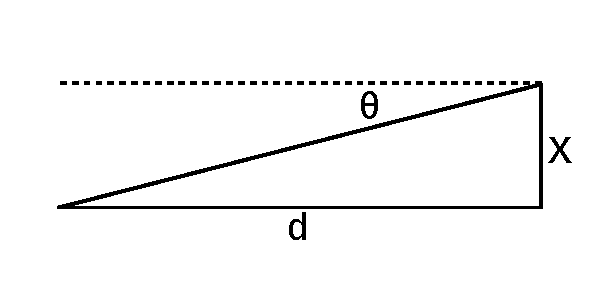
\includegraphics[width=0.25\textwidth]{CompassTriangle.pdf}
\caption{\label{fig:triang} A basic diagram of the triangulation we've performed by walking the baseline $x$ to obtain the distance $d$.}
\end{figure}

This week we have obtained compass data from a baseline hike that will allow us to calculate the distance to the center of Los Angeles, \textit{without walking all the way there.}  Consult Fig. \ref{fig:triang}, which contains a diagram with the essential parameters of this calculation.  The variable $x$ is the baseline we walked to the water tower in Hellman Park.  From the top of the Science and Learning Center, the straight-line distance to the water tower is $x = 3.13$ km.  From the water tower, we measured the compass angle to the center of downtown Los Angeles.  Let's take this angle to correspond to the side $d$ in Fig. \ref{fig:triang}.  We also measured the compass heading from the Science and Learning Center.  Let the heading from the hill be $\theta_1$ and the heading from SLC be $\theta_2$.  It turns out that 

\begin{equation}
\theta = \theta_1 - \theta_2
\end{equation}

The small angle of the triangle (from the properties of parallel lines) also turns out to be equal to $\theta$.  Convince yourself that 

\begin{align}
\tan\theta &= \frac{x}{d} \\
d &= \frac{x}{\tan\theta} \label{eq:theone}
\end{align}

Here's the problem: if we all plug in our different answers for $\theta_1$ and $\theta_2$, we'll get different distances to downtown Los Angeles.

\section{Averaging}

Share at your table your different measurements for $\theta_1$ and $\theta_2$.  Compute the \textit{average} of each value, in degrees, and record them below.  \\ \vspace{0.5cm}

Now record your group's answer for the $\theta$, or the difference between the two angles below. \\ \vspace{0.5cm}

\section{The Distance}

Using Eq. \ref{eq:theone}, calculate the distance to downtown Los Angeles, and record your answer below.  Compare to other groups, and check the real answer on Google Maps.  How close to the true result are we?

\end{document}
